\begingroup
\setstretch{1}
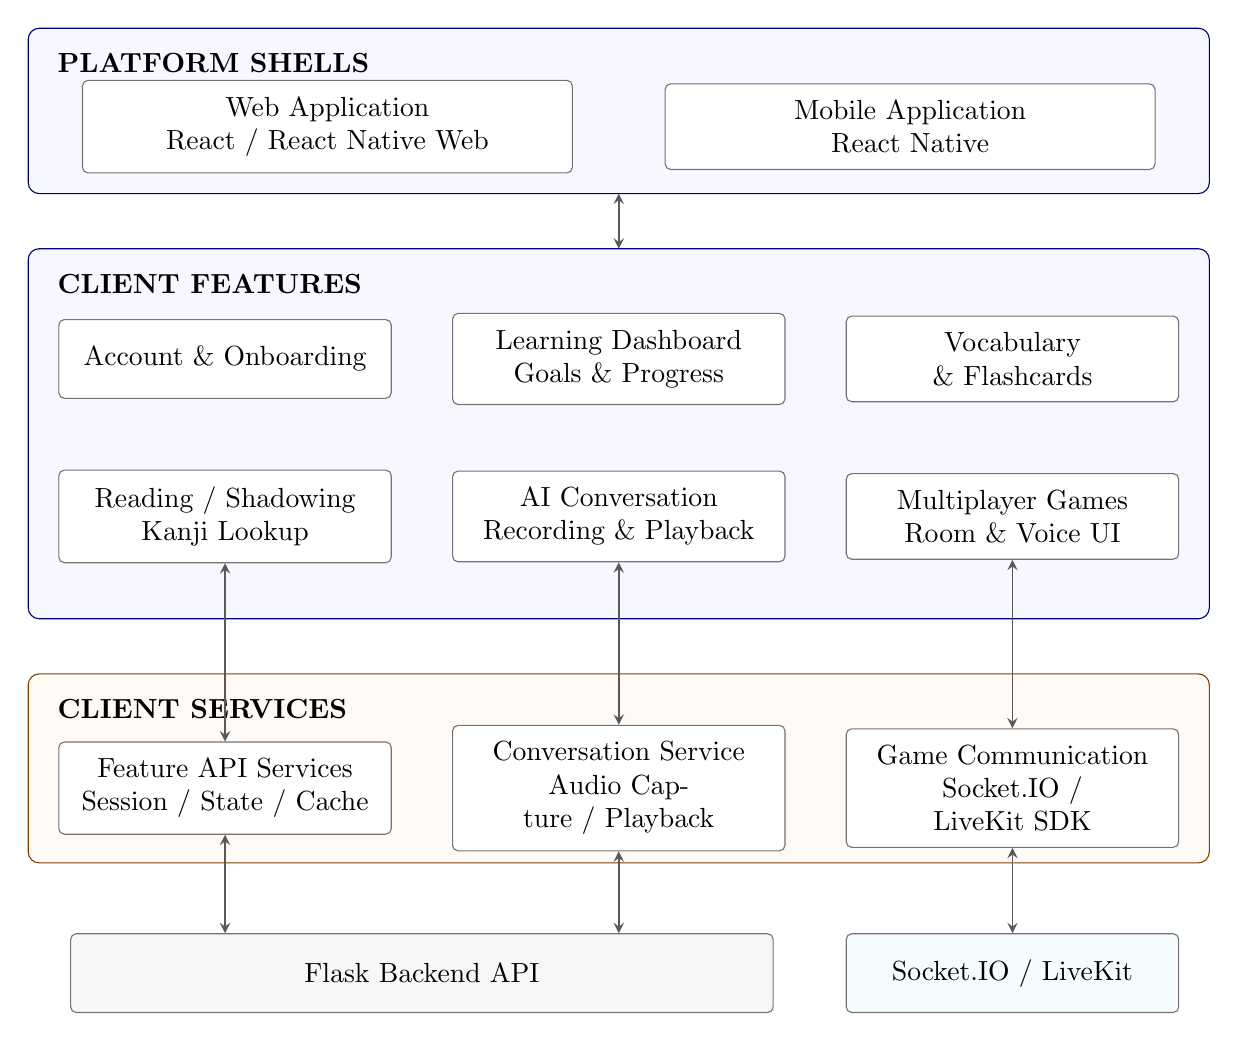
\begin{tikzpicture}[
box/.style={draw=black!55,rounded corners=2pt,fill=white,text width=3.8cm,minimum height=1cm,inner sep=6pt,align=center,font=\fontsize{10}{12}\selectfont},
title/.style={anchor=north west,font=\fontsize{10}{12}\selectfont\bfseries},
link/.style={<->,>=stealth,draw=black!65,line width=.65pt,rounded corners=3pt},
task/.style={->,>=stealth,draw=black!65,line width=.65pt,rounded corners=3pt}]

\draw[rounded corners,draw=blue!45!black,fill=blue!3] (-7.5,0) rectangle (7.5,-2.1);
\node[title] at (-7.25,-.2) {PLATFORM SHELLS};
\node[box,text width=5.8cm] at (-3.7,-1.25) {Web Application\\React / React Native Web};
\node[box,text width=5.8cm] at (3.7,-1.25) {Mobile Application\\React Native};
\draw[rounded corners,draw=blue!45!black,fill=blue!3] (-7.5,-2.8) rectangle (7.5,-7.5);
\node[title] at (-7.25,-3) {CLIENT FEATURES};
\node[box] at (-5,-4.2) {Account \& Onboarding};
\node[box] at (0,-4.2) {Learning Dashboard\\Goals \& Progress};
\node[box] at (5,-4.2) {Vocabulary \& Flashcards};
\node[box] (learning) at (-5,-6.2) {Reading / Shadowing\\Kanji Lookup};
\node[box] (speaking) at (0,-6.2) {AI Conversation\\Recording \& Playback};
\node[box] (games) at (5,-6.2) {Multiplayer Games\\Room \& Voice UI};
\draw[link] (0,-2.1) -- (0,-2.8);
\draw[rounded corners,draw=orange!50!black,fill=orange!4] (-7.5,-8.2) rectangle (7.5,-10.6);
\node[title] at (-7.25,-8.4) {CLIENT SERVICES};
\node[box] (api) at (-5,-9.65) {Feature API Services\\Session / State / Cache};
\node[box] (voice) at (0,-9.65) {Conversation Service\\Audio Capture / Playback};
\node[box] (realtime) at (5,-9.65) {Game Communication\\Socket.IO / LiveKit SDK};
\draw[link] (learning.south) -- (api.north);
\draw[link] (speaking.south) -- (voice.north);
\draw[link] (games.south) -- (realtime.north);
\node[box,text width=8.5cm,fill=black!3] (server) at (-2.5,-12) {Flask Backend API};
\node[box,fill=cyan!4] (media) at (5,-12) {Socket.IO / LiveKit};
\draw[link] (api.south) -- (-5,0 |- server.north);
\draw[link] (voice.south) -- (0,0 |- server.north);
\draw[link] (realtime.south) -- (media.north);
\end{tikzpicture}
\endgroup
